% Topic T1.4: Landscape Overview
% Self-contained Beamer slides for Digital Finance course
\documentclass[11pt,aspectratio=169]{beamer}
\usetheme{Madrid}

% ======================= PACKAGES =======================
\usepackage{graphicx}
\usepackage{booktabs}
\usepackage{adjustbox}
\usepackage{multicol}
\usepackage{amsmath}
\usepackage{amssymb}
\usepackage{tikz}
\usetikzlibrary{arrows,shapes,positioning,shadows,trees}
\usepackage{listings}
\usepackage{xcolor}

% ======================= COLOR DEFINITIONS =======================
% Primary color scheme: Blue/Teal for Digital Finance
\definecolor{dfblue}{RGB}{0,102,204}
\definecolor{dfteal}{RGB}{0,153,153}
\definecolor{dfcyan}{RGB}{51,187,204}
\definecolor{dflightblue}{RGB}{153,204,255}
\definecolor{dflightblue2}{RGB}{173,214,255}
\definecolor{dflightblue3}{RGB}{193,224,255}
\definecolor{dflightblue4}{RGB}{213,234,255}

% Accent colors for finance applications
\definecolor{dfgreen}{RGB}{44, 160, 44}
\definecolor{dfred}{RGB}{214, 39, 40}
\definecolor{dforange}{RGB}{255, 127, 14}
\definecolor{dfgray}{RGB}{127, 127, 127}

% Utility colors
\definecolor{lightgray}{RGB}{240, 240, 240}
\definecolor{midgray}{RGB}{180, 180, 180}
\definecolor{codebg}{RGB}{245, 245, 245}

% ======================= THEME CUSTOMIZATION =======================
% Apply Digital Finance color scheme to Madrid theme
\setbeamercolor{palette primary}{bg=dflightblue3,fg=dfblue}
\setbeamercolor{palette secondary}{bg=dflightblue2,fg=dfblue}
\setbeamercolor{palette tertiary}{bg=dfteal,fg=white}
\setbeamercolor{palette quaternary}{bg=dfblue,fg=white}

\setbeamercolor{structure}{fg=dfblue}
\setbeamercolor{section in toc}{fg=dfblue}
\setbeamercolor{subsection in toc}{fg=dfteal}
\setbeamercolor{title}{fg=dfblue}
\setbeamercolor{frametitle}{fg=dfblue,bg=dflightblue3}
\setbeamercolor{block title}{bg=dflightblue2,fg=dfblue}
\setbeamercolor{block body}{bg=dflightblue4,fg=black}

% Remove navigation symbols for cleaner look
\setbeamertemplate{navigation symbols}{}

% Clean itemize/enumerate
\setbeamertemplate{itemize items}[circle]
\setbeamertemplate{enumerate items}[default]

% Margins for readability
\setbeamersize{text margin left=8mm,text margin right=8mm}

% ======================= LISTINGS CONFIGURATION =======================
% Python code style
\lstdefinestyle{pythonstyle}{
    language=Python,
    basicstyle=\ttfamily\footnotesize,
    keywordstyle=\color{dfblue}\bfseries,
    stringstyle=\color{dforange},
    commentstyle=\color{dfgray}\itshape,
    numberstyle=\tiny\color{dfgray},
    numbers=left,
    numbersep=5pt,
    backgroundcolor=\color{codebg},
    showspaces=false,
    showstringspaces=false,
    showtabs=false,
    frame=single,
    rulecolor=\color{midgray},
    tabsize=4,
    captionpos=b,
    breaklines=true,
    breakatwhitespace=false,
    escapeinside={(*@}{@*)},
    xleftmargin=10pt,
    xrightmargin=10pt
}

% Solidity code style
\lstdefinestyle{soliditystyle}{
    language=Java, % closest approximation
    basicstyle=\ttfamily\footnotesize,
    keywordstyle=\color{dfteal}\bfseries,
    stringstyle=\color{dforange},
    commentstyle=\color{dfgray}\itshape,
    numberstyle=\tiny\color{dfgray},
    numbers=left,
    numbersep=5pt,
    backgroundcolor=\color{codebg},
    showspaces=false,
    showstringspaces=false,
    showtabs=false,
    frame=single,
    rulecolor=\color{midgray},
    tabsize=2,
    captionpos=b,
    breaklines=true,
    breakatwhitespace=false,
    escapeinside={(*@}{@*)},
    xleftmargin=10pt,
    xrightmargin=10pt,
    morekeywords={pragma, contract, function, returns, public, private, view, pure, payable, address, uint256, mapping, event, modifier}
}

% Inline code command
\newcommand{\code}[1]{\texttt{\color{dfblue}#1}}

% ======================= CUSTOM COMMANDS =======================
% Bottom annotation (Madrid-style)
\newcommand{\bottomnote}[1]{%
\vfill
\vspace{-2mm}
\textcolor{dflightblue2}{\rule{\textwidth}{0.4pt}}
\vspace{1mm}
\footnotesize
\textbf{#1}
}

% Compact list spacing
\newcommand{\compactlist}{%
\setlength{\itemsep}{0pt}%
\setlength{\parskip}{0pt}%
\setlength{\parsep}{0pt}%
}

% Chart placeholder
\newcommand{\chartplaceholder}[2][5cm]{%
\begin{center}
\begin{adjustbox}{max width=0.95\textwidth, max height=#1}
\framebox[\textwidth][c]{%
\rule{0pt}{#1}%
\textcolor{midgray}{[#2]}%
}
\end{adjustbox}
\end{center}
}

% ======================= FINANCE NOTATION MACROS =======================
% Probability and statistics
\newcommand{\E}{\mathbb{E}} % Expected value
\newcommand{\Var}{\mathrm{Var}} % Variance
\newcommand{\Cov}{\mathrm{Cov}} % Covariance
\newcommand{\Prob}{\mathbb{P}} % Probability

% Distributions
\newcommand{\Normal}{\mathcal{N}} % Normal distribution
\newcommand{\Uniform}{\mathcal{U}} % Uniform distribution

% Returns and prices
\newcommand{\Ret}{R} % Return
\newcommand{\LogRet}{r} % Log return
\newcommand{\Price}{S} % Price/Stock price
\newcommand{\Strike}{K} % Strike price

% Options and derivatives
\newcommand{\CallPrice}{C} % Call option price
\newcommand{\PutPrice}{P} % Put option price
\newcommand{\Greeks}[1]{\mathit{#1}} % Greek letters

% Risk measures
\newcommand{\VaR}{\mathrm{VaR}} % Value at Risk
\newcommand{\CVaR}{\mathrm{CVaR}} % Conditional VaR
\newcommand{\Sharpe}{\mathrm{SR}} % Sharpe Ratio

% Time series
\newcommand{\AR}{\mathrm{AR}} % Autoregressive
\newcommand{\MA}{\mathrm{MA}} % Moving average
\newcommand{\GARCH}{\mathrm{GARCH}} % GARCH

% Blockchain/Crypto
\newcommand{\Hash}{\mathrm{Hash}} % Hash function
\newcommand{\Block}{\mathcal{B}} % Block
\newcommand{\Chain}{\mathcal{C}} % Chain

% Real numbers, integers
\newcommand{\R}{\mathbb{R}}
\newcommand{\Z}{\mathbb{Z}}
\newcommand{\N}{\mathbb{N}}

% ======================= TIKZ STYLES =======================
% Styles for finance-related diagrams
\tikzstyle{process} = [rectangle, minimum width=3cm, minimum height=1cm, text centered, draw=dfblue, fill=dflightblue4, thick]
\tikzstyle{decision} = [diamond, minimum width=3cm, minimum height=1cm, text centered, draw=dfteal, fill=dflightblue4, thick]
\tikzstyle{arrow} = [thick,->,>=stealth,color=dfblue]
\tikzstyle{blockchain} = [rectangle, rounded corners, minimum width=2.5cm, minimum height=1cm, text centered, draw=dfteal, fill=dflightblue3, thick]
\tikzstyle{transaction} = [circle, minimum size=0.8cm, text centered, draw=dforange, fill=dflightblue4, thick]

% ======================= FOOTER TEMPLATE =======================
\setbeamertemplate{footline}{
    \hbox{\begin{beamercolorbox}[wd=\paperwidth,ht=2.5ex,dp=1ex,leftskip=.5em,rightskip=.5em]{author in head/foot}
    \tiny
    \textbf{Digital Finance} \hfill
    Joerg Osterrieder \hfill
    \insertdate \hfill
    Page \insertframenumber{} / \inserttotalframenumber
    \end{beamercolorbox}}
}

% ======================= SECTION DIVIDER TEMPLATE =======================
\AtBeginSection[]{
\begin{frame}[plain]
\vfill
\centering
\begin{beamercolorbox}[sep=12pt,center]{title}
\usebeamerfont{title}\LARGE\insertsection\par
\end{beamercolorbox}
\vfill
\end{frame}
}


\title[T1.4: Landscape]{Topic 1.4: Digital Finance Landscape}
\subtitle{A Map of Digital Finance}
\author{Joerg Osterrieder}
\institute{Digital Finance}
\date{2025}

\begin{document}

% ==================== SLIDE 1: Title ====================
\begin{frame}[plain]
\titlepage
\end{frame}

% ==================== SLIDE 2: Learning Objectives ====================
\begin{frame}{Learning Objectives}
\begin{center}
\textbf{\Large What You Will Learn in This Topic}
\end{center}

\vspace{5mm}
By the end of this section, you will be able to:
\begin{enumerate}
\item \textbf{Visualize} the full scope of digital finance as an interconnected ecosystem
\item \textbf{Understand} how different sectors connect and depend on each other
\item \textbf{Locate} any innovation within the landscape framework
\item \textbf{Distinguish} between infrastructure and application layers
\item \textbf{Navigate} the six core sectors of digital finance
\item \textbf{Anticipate} where emerging categories are heading
\end{enumerate}

\vspace{5mm}
\begin{block}{Why a Map Matters}
Without structure, digital finance seems like ``a collection of cool things.''\\
A map lets you see patterns, gaps, and connections.
\end{block}
\end{frame}

% ==================== SLIDE 3: Prerequisites ====================
\begin{frame}{Prerequisites and Background}
\begin{columns}[T]
\begin{column}{0.48\textwidth}
\textbf{What You Should Already Know:}
\begin{itemize}
\item Basic understanding of traditional finance
\item The concept of financial friction
\item FinTech vs. Crypto/DeFi philosophies
\item How trust operates in financial systems
\end{itemize}

\vspace{3mm}
\textbf{From Previous Topics:}
\begin{itemize}
\item T1.1: Money as trust infrastructure
\item T1.2: Financial friction points
\item T1.3: Two approaches to innovation
\end{itemize}
\end{column}
\begin{column}{0.48\textwidth}
\textbf{Key Concepts to Review:}
\begin{itemize}
\item \textbf{Friction} = opportunity for innovation
\item \textbf{Intermediation} vs. disintermediation
\item \textbf{Rails} = the underlying infrastructure
\item \textbf{UX} = user experience layer
\end{itemize}

\vspace{3mm}
\begin{alertblock}{Mental Model}
Think of digital finance like a city:\\
Sectors = neighborhoods\\
Infrastructure = roads and utilities\\
Applications = buildings and businesses
\end{alertblock}
\end{column}
\end{columns}
\end{frame}

% ==================== SLIDE 4: Framework Introduction ====================
\begin{frame}{The Landscape Framework}
\begin{center}
\textbf{\Large How We Organize Digital Finance}
\end{center}

\vspace{3mm}
\begin{columns}[T]
\begin{column}{0.48\textwidth}
\textbf{Three Organizing Principles:}
\begin{enumerate}
\item \textbf{By Function:} What problem does it solve?
\item \textbf{By Technology:} What rails does it use?
\item \textbf{By User:} Who benefits?
\end{enumerate}

\vspace{3mm}
\textbf{The Six Core Sectors:}
\begin{enumerate}
\item Payments
\item Lending
\item Trading \& Exchanges
\item Investing \& Wealth Management
\item Insurance
\item Banking Infrastructure
\end{enumerate}

\vspace{2mm}
\begin{alertblock}{First-Time Learner Note}
We'll explore each sector in detail -- don't try to memorize everything now. Just get the big picture of how digital finance is organized.
\end{alertblock}
\end{column}
\begin{column}{0.48\textwidth}
\textbf{Key Insight:}
\begin{itemize}
\item Every sector exists in both FinTech and Crypto/DeFi forms
\item Infrastructure underlies all sectors
\item Sectors interconnect and depend on each other
\item Emerging categories blur sector boundaries
\end{itemize}

\vspace{3mm}
\begin{block}{Framework Value}
This framework lets you place ANY digital finance innovation in context and understand its relationships.
\end{block}
\end{column}
\end{columns}
\end{frame}

% ==================== SLIDE 5: The Digital Finance Landscape ====================
\begin{frame}{The Digital Finance Landscape}
\begin{center}
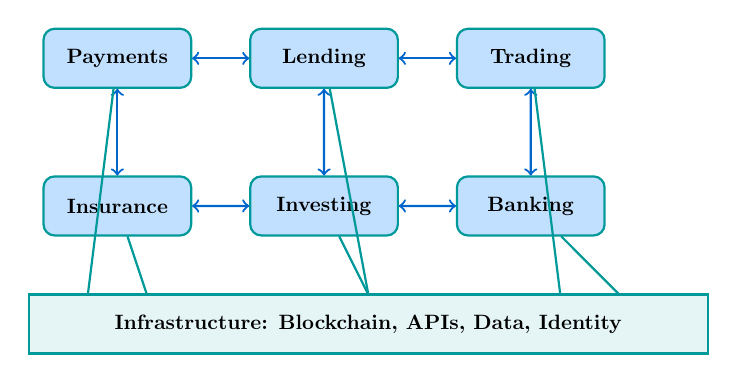
\begin{tikzpicture}[scale=0.75, transform shape]
% Main categories
\node (payments) [blockchain, minimum width=2.5cm, minimum height=1cm] {\textbf{Payments}};
\node (lending) [blockchain, right of=payments, node distance=3.5cm, minimum width=2.5cm, minimum height=1cm] {\textbf{Lending}};
\node (trading) [blockchain, right of=lending, node distance=3.5cm, minimum width=2.5cm, minimum height=1cm] {\textbf{Trading}};

\node (insurance) [blockchain, below of=payments, node distance=2.5cm, minimum width=2.5cm, minimum height=1cm] {\textbf{Insurance}};
\node (invest) [blockchain, below of=lending, node distance=2.5cm, minimum width=2.5cm, minimum height=1cm] {\textbf{Investing}};
\node (banking) [blockchain, below of=trading, node distance=2.5cm, minimum width=2.5cm, minimum height=1cm] {\textbf{Banking}};

% Infrastructure layer
\draw[thick, dfteal, fill=dfteal!10] (-1.5,-4) rectangle (10,-5);
\node at (4.25,-4.5) {\textbf{Infrastructure: Blockchain, APIs, Data, Identity}};

% Connections
\draw[thick, dfblue, <->] (payments) -- (lending);
\draw[thick, dfblue, <->] (lending) -- (trading);
\draw[thick, dfblue, <->] (payments) -- (insurance);
\draw[thick, dfblue, <->] (lending) -- (invest);
\draw[thick, dfblue, <->] (trading) -- (banking);
\draw[thick, dfblue, <->] (insurance) -- (invest);
\draw[thick, dfblue, <->] (invest) -- (banking);

% Connect to infrastructure
\draw[thick, dfteal] (payments) -- (-0.5,-4);
\draw[thick, dfteal] (insurance) -- (0.5,-4);
\draw[thick, dfteal] (lending) -- (4.25,-4);
\draw[thick, dfteal] (invest) -- (4.25,-4);
\draw[thick, dfteal] (trading) -- (7.5,-4);
\draw[thick, dfteal] (banking) -- (8.5,-4);
\end{tikzpicture}
\end{center}

\vspace{3mm}
\textbf{Key observation:} All sectors are interconnected. A payment enables a trade, which may fund a loan, which may provide collateral for insurance.
\end{frame}

% ==================== SLIDE 6: Sector 1 - Payments Overview ====================
\begin{frame}{Sector 1: Payments}
\begin{columns}[T]
\begin{column}{0.48\textwidth}
\textbf{What it covers:}
\begin{itemize}
\item Person-to-person (P2P)
\item Consumer-to-business (C2B)
\item Business-to-business (B2B)
\item Cross-border remittances
\item Point-of-sale systems
\item Digital wallets
\end{itemize}

\vspace{3mm}
\textbf{Key friction addressed:}\\
Speed, cost, convenience
\end{column}
\begin{column}{0.48\textwidth}
\textbf{FinTech examples:}
\begin{itemize}
\item Venmo, Zelle, Cash App
\item Stripe, Square, Adyen
\item Wise, Remitly
\end{itemize}

\vspace{3mm}
\textbf{Crypto examples:}
\begin{itemize}
\item Bitcoin Lightning
\item USDC/USDT transfers
\item Solana Pay
\end{itemize}
\end{column}
\end{columns}

\vspace{3mm}
\begin{block}{Simple Examples You Know}
\textbf{P2P:} Venmo, PayPal sending money to friends\\
\textbf{C2B:} Apple Pay at Starbucks, buying online\\
\textbf{Cross-border:} Sending money home to family abroad
\end{block}

\vspace{2mm}
\begin{block}{Coming in Day 2}
Deep dive into payment infrastructure, rails, and the future of money movement.
\end{block}
\end{frame}

% ==================== SLIDE 7: Payments Deep Dive ====================
\begin{frame}{Payments: The Foundation of Finance}
\begin{center}
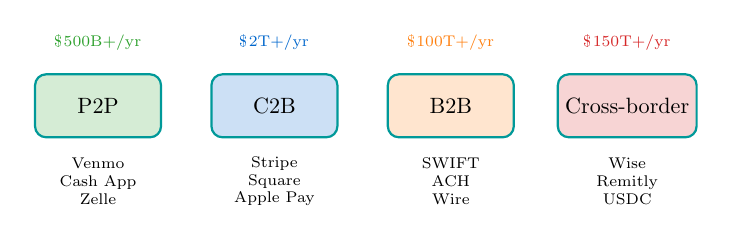
\begin{tikzpicture}[scale=0.8, transform shape]
% Payment types
\node (p2p) [blockchain, minimum width=2cm, fill=dfgreen!20] {P2P};
\node (c2b) [blockchain, right of=p2p, node distance=2.8cm, minimum width=2cm, fill=dfblue!20] {C2B};
\node (b2b) [blockchain, right of=c2b, node distance=2.8cm, minimum width=2cm, fill=dforange!20] {B2B};
\node (cross) [blockchain, right of=b2b, node distance=2.8cm, minimum width=2cm, fill=dfred!20] {Cross-border};

% Examples below
\node[below of=p2p, node distance=1.2cm, font=\scriptsize, text width=2cm, align=center] {Venmo\\Cash App\\Zelle};
\node[below of=c2b, node distance=1.2cm, font=\scriptsize, text width=2cm, align=center] {Stripe\\Square\\Apple Pay};
\node[below of=b2b, node distance=1.2cm, font=\scriptsize, text width=2cm, align=center] {SWIFT\\ACH\\Wire};
\node[below of=cross, node distance=1.2cm, font=\scriptsize, text width=2.3cm, align=center] {Wise\\Remitly\\USDC};

% Volume indicators
\node[above of=p2p, node distance=1cm, font=\scriptsize, text=dfgreen] {\$500B+/yr};
\node[above of=c2b, node distance=1cm, font=\scriptsize, text=dfblue] {\$2T+/yr};
\node[above of=b2b, node distance=1cm, font=\scriptsize, text=dforange] {\$100T+/yr};
\node[above of=cross, node distance=1cm, font=\scriptsize, text=dfred] {\$150T+/yr};
\end{tikzpicture}
\end{center}

\vspace{3mm}
\textbf{Why Payments Matter Most:}
\begin{itemize}
\item Entry point for most users into digital finance
\item Highest transaction volume of any sector
\item Foundation for all other financial activities
\item Fastest innovation cycle
\end{itemize}
\end{frame}

% ==================== SLIDE 8: Payments Innovation Spectrum ====================
\begin{frame}{Payments: Innovation Spectrum}
\begin{center}
\textbf{From Traditional to Revolutionary}
\end{center}

\vspace{3mm}
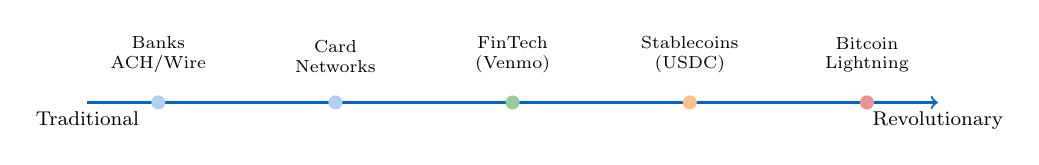
\begin{tikzpicture}[scale=0.9, transform shape]
% Spectrum line
\draw[thick, ->, dfblue] (0,0) -- (12,0);
\node[below] at (0,0) {\footnotesize Traditional};
\node[below] at (12,0) {\footnotesize Revolutionary};

% Points on spectrum
\node[above, text width=2cm, align=center, font=\scriptsize] at (1,0.3) {Banks\\ACH/Wire};
\node[fill=dfblue!30, circle, inner sep=2pt] at (1,0) {};

\node[above, text width=2cm, align=center, font=\scriptsize] at (3.5,0.3) {Card\\Networks};
\node[fill=dfblue!30, circle, inner sep=2pt] at (3.5,0) {};

\node[above, text width=2cm, align=center, font=\scriptsize] at (6,0.3) {FinTech\\(Venmo)};
\node[fill=dfgreen!50, circle, inner sep=2pt] at (6,0) {};

\node[above, text width=2cm, align=center, font=\scriptsize] at (8.5,0.3) {Stablecoins\\(USDC)};
\node[fill=dforange!50, circle, inner sep=2pt] at (8.5,0) {};

\node[above, text width=2cm, align=center, font=\scriptsize] at (11,0.3) {Bitcoin\\Lightning};
\node[fill=dfred!50, circle, inner sep=2pt] at (11,0) {};
\end{tikzpicture}

\vspace{5mm}
\begin{columns}[T]
\begin{column}{0.48\textwidth}
\textbf{FinTech Approach:}
\begin{itemize}
\item Better UX on existing rails
\item Instant P2P (funded by float)
\item Lower merchant fees
\item Mobile-first experience
\end{itemize}
\end{column}
\begin{column}{0.48\textwidth}
\textbf{Crypto Approach:}
\begin{itemize}
\item New settlement layer
\item 24/7/365 availability
\item Borderless by design
\item Programmable payments
\end{itemize}
\end{column}
\end{columns}
\end{frame}

% ==================== SLIDE 9: Sector 2 - Lending Overview ====================
\begin{frame}{Sector 2: Lending}
\begin{columns}[T]
\begin{column}{0.48\textwidth}
\textbf{What it covers:}
\begin{itemize}
\item Consumer lending
\item SMB lending
\item Peer-to-peer lending
\item Buy-now-pay-later (BNPL)
\item Collateralized lending
\item Flash loans
\end{itemize}

\vspace{3mm}
\textbf{Key friction addressed:}\\
Access, speed, cost of credit
\end{column}
\begin{column}{0.48\textwidth}
\textbf{FinTech examples:}
\begin{itemize}
\item LendingClub, Upstart
\item Affirm, Klarna, Afterpay
\item Kabbage, Funding Circle
\end{itemize}

\vspace{3mm}
\textbf{Crypto examples:}
\begin{itemize}
\item Aave, Compound
\item MakerDAO (DAI)
\item Liquity, Euler
\end{itemize}
\end{column}
\end{columns}

\vspace{3mm}
\begin{alertblock}{Embedded Finance Example}
\textbf{Buy Now, Pay Later} at checkout -- Klarna, Afterpay, Affirm built into shopping sites. No credit card needed, split purchases into installments.\\
\textbf{Others:} Insurance when booking a flight, loans offered at car dealerships.
\end{alertblock}

\vspace{2mm}
\begin{block}{Coming in Days 2 \& 4}
Platform-based lending (Day 2), DeFi lending protocols (Day 4).
\end{block}
\end{frame}

% ==================== SLIDE 10: Lending Deep Dive ====================
\begin{frame}{Lending: Credit Innovation}
\begin{center}
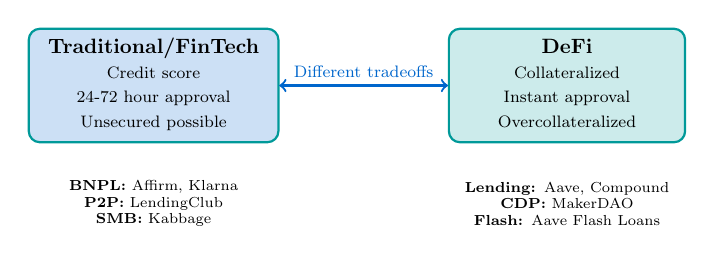
\begin{tikzpicture}[scale=0.75, transform shape]
% Traditional vs DeFi comparison
\node[blockchain, minimum width=4cm, fill=dfblue!20] (trad) at (0,0) {
\begin{tabular}{c}
\textbf{Traditional/FinTech}\\
\footnotesize Credit score\\
\footnotesize 24-72 hour approval\\
\footnotesize Unsecured possible
\end{tabular}
};

\node[blockchain, minimum width=4cm, fill=dfteal!20] (defi) at (7,0) {
\begin{tabular}{c}
\textbf{DeFi}\\
\footnotesize Collateralized\\
\footnotesize Instant approval\\
\footnotesize Overcollateralized
\end{tabular}
};

% Arrow with question
\draw[thick, <->, dfblue] (trad) -- (defi) node[midway, above] {\footnotesize Different tradeoffs};

% Examples below
\node[below of=trad, node distance=2cm, font=\scriptsize, text width=4cm, align=center] {
\textbf{BNPL:} Affirm, Klarna\\
\textbf{P2P:} LendingClub\\
\textbf{SMB:} Kabbage
};

\node[below of=defi, node distance=2cm, font=\scriptsize, text width=4cm, align=center] {
\textbf{Lending:} Aave, Compound\\
\textbf{CDP:} MakerDAO\\
\textbf{Flash:} Aave Flash Loans
};
\end{tikzpicture}
\end{center}

\vspace{3mm}
\textbf{Key Innovation:} Alternative credit scoring (FinTech) and trustless collateral (DeFi) both expand access to credit beyond traditional banks.
\end{frame}

% ==================== SLIDE 11: BNPL Explained ====================
\begin{frame}{BNPL: Buy Now, Pay Later}
\begin{center}
\textbf{\Large The Fastest-Growing Lending Category}
\end{center}

\vspace{3mm}
\begin{columns}[T]
\begin{column}{0.48\textwidth}
\textbf{How BNPL Works:}
\begin{enumerate}
\item Customer selects BNPL at checkout
\item BNPL provider pays merchant (minus fee)
\item Customer pays BNPL in 4-6 installments
\item Often 0\% APR if paid on time
\end{enumerate}

\vspace{3mm}
\textbf{Major Players:}
\begin{itemize}
\item Affirm (US)
\item Klarna (Europe)
\item Afterpay (Australia/Block)
\end{itemize}
\end{column}
\begin{column}{0.48\textwidth}
\textbf{Why It's Disrupting Credit Cards:}
\begin{itemize}
\item Transparent fees
\item No compound interest
\item Instant approval
\item Popular with Gen Z/Millennials
\end{itemize}

\vspace{3mm}
\begin{alertblock}{Risk Factor}
Defaults rising as interest rates increase. Regulatory scrutiny growing. Credit reporting rules changing.
\end{alertblock}
\end{column}
\end{columns}
\end{frame}

% ==================== SLIDE 12: Sector 3 - Trading ====================
\begin{frame}{Sector 3: Trading \& Exchanges}
\begin{columns}[T]
\begin{column}{0.48\textwidth}
\textbf{What it covers:}
\begin{itemize}
\item Stock trading
\item Crypto exchanges
\item Derivatives
\item Forex
\item NFT marketplaces
\item Tokenized assets
\end{itemize}

\vspace{3mm}
\textbf{Key friction addressed:}\\
Access, fees, transparency
\end{column}
\begin{column}{0.48\textwidth}
\textbf{FinTech examples:}
\begin{itemize}
\item Robinhood, Webull, eToro
\item Interactive Brokers
\item Public, Alpaca
\end{itemize}

\vspace{3mm}
\textbf{Crypto examples:}
\begin{itemize}
\item Uniswap, Curve, Balancer
\item dYdX, GMX
\item OpenSea, Blur
\end{itemize}
\end{column}
\end{columns}

\vspace{3mm}
\begin{alertblock}{Sector Boundaries are Fluid}
Many companies span multiple sectors -- PayPal does payments AND lending AND crypto. Uber offers both payment services and driver banking. This overlap is a feature, not a bug.
\end{alertblock}

\vspace{2mm}
\begin{block}{Coming in Days 3 \& 4}
Decentralized exchanges and AMMs (Days 3-4), trading mechanics.
\end{block}
\end{frame}

% ==================== SLIDE 13: CEX vs DEX ====================
\begin{frame}{Trading: CEX vs. DEX}
\begin{center}
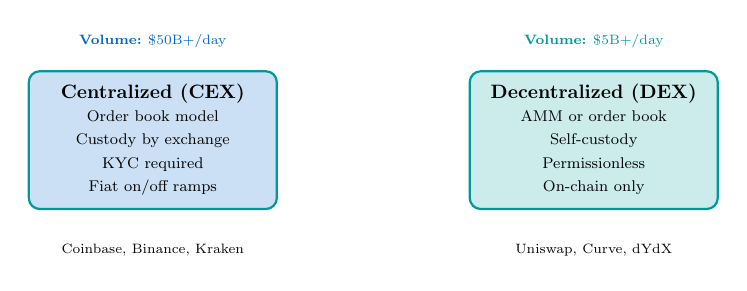
\begin{tikzpicture}[scale=0.7, transform shape]
% CEX side
\node[blockchain, minimum width=4.5cm, minimum height=2.5cm, fill=dfblue!20] (cex) at (0,0) {
\begin{tabular}{c}
\textbf{Centralized (CEX)}\\
\footnotesize Order book model\\
\footnotesize Custody by exchange\\
\footnotesize KYC required\\
\footnotesize Fiat on/off ramps
\end{tabular}
};

% DEX side
\node[blockchain, minimum width=4.5cm, minimum height=2.5cm, fill=dfteal!20] (dex) at (8,0) {
\begin{tabular}{c}
\textbf{Decentralized (DEX)}\\
\footnotesize AMM or order book\\
\footnotesize Self-custody\\
\footnotesize Permissionless\\
\footnotesize On-chain only
\end{tabular}
};

% Examples
\node[below of=cex, node distance=2cm, font=\scriptsize] {Coinbase, Binance, Kraken};
\node[below of=dex, node distance=2cm, font=\scriptsize] {Uniswap, Curve, dYdX};

% Volume comparison
\node[above of=cex, node distance=1.8cm, font=\scriptsize, text=dfblue] {\textbf{Volume:} \$50B+/day};
\node[above of=dex, node distance=1.8cm, font=\scriptsize, text=dfteal] {\textbf{Volume:} \$5B+/day};
\end{tikzpicture}
\end{center}

\vspace{3mm}
\textbf{Key Distinction:} CEX = convenience and fiat access; DEX = self-custody and permissionless trading.
\end{frame}

% ==================== SLIDE 14: AMM Explained ====================
\begin{frame}{Trading Innovation: Automated Market Makers}
\begin{center}
\textbf{How DEXs Work Without Order Books}
\end{center}

\vspace{3mm}
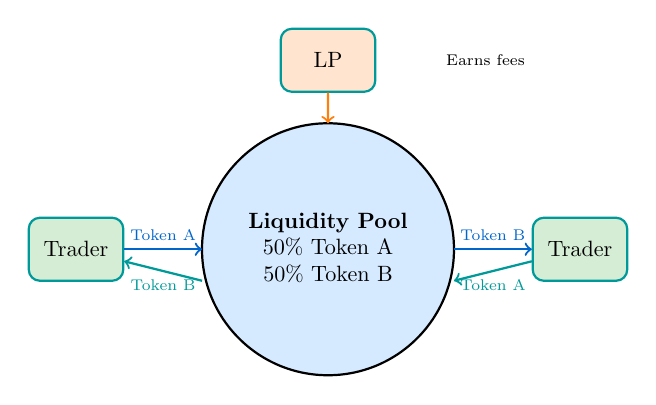
\begin{tikzpicture}[scale=0.8, transform shape]
% Liquidity pool
\draw[thick, fill=dflightblue4] (4,0) circle (2cm);
\node at (4,0) {
\begin{tabular}{c}
\textbf{Liquidity Pool}\\
50\% Token A\\
50\% Token B
\end{tabular}
};

% Traders
\node[blockchain, minimum width=1.5cm, fill=dfgreen!20] (trader1) at (0,0) {Trader};
\node[blockchain, minimum width=1.5cm, fill=dfgreen!20] (trader2) at (8,0) {Trader};

% Arrows
\draw[thick, ->, dfblue] (trader1) -- (2,0) node[midway, above, font=\scriptsize] {Token A};
\draw[thick, <-, dfteal] (trader1) -- (2,-0.5) node[midway, below, font=\scriptsize] {Token B};

\draw[thick, <-, dfblue] (trader2) -- (6,0) node[midway, above, font=\scriptsize] {Token B};
\draw[thick, ->, dfteal] (trader2) -- (6,-0.5) node[midway, below, font=\scriptsize] {Token A};

% LP providers
\node[blockchain, minimum width=1.5cm, fill=dforange!20] (lp) at (4,3) {LP};
\draw[thick, ->, dforange] (lp) -- (4,2);
\node[right of=lp, node distance=2.5cm, font=\scriptsize] {Earns fees};
\end{tikzpicture}

\vspace{3mm}
\textbf{Formula:} $x \times y = k$ (constant product)

Liquidity providers deposit assets, earn trading fees. Prices adjust automatically based on supply/demand.
\end{frame}

% ==================== SLIDE 15: Sector 4 - Investing ====================
\begin{frame}{Sector 4: Investing \& Wealth Management}
\begin{columns}[T]
\begin{column}{0.48\textwidth}
\textbf{What it covers:}
\begin{itemize}
\item Robo-advisors
\item Fractional investing
\item Micro-investing
\item Alternative investments
\item Portfolio management
\item Yield aggregation
\end{itemize}

\vspace{3mm}
\textbf{Key friction addressed:}\\
Minimums, expertise, access
\end{column}
\begin{column}{0.48\textwidth}
\textbf{FinTech examples:}
\begin{itemize}
\item Betterment, Wealthfront
\item Acorns, Stash
\item Fundrise, Republic
\end{itemize}

\vspace{3mm}
\textbf{Crypto examples:}
\begin{itemize}
\item Yearn Finance
\item Index Coop
\item Enzyme Finance
\end{itemize}
\end{column}
\end{columns}

\vspace{3mm}
\begin{alertblock}{Fractional Ownership Revolution}
\textbf{Tokenization} lets you own 1\% of a Picasso painting, or \$100 worth of a commercial building. Previously, you needed millions to invest in real estate or art. Now, accessible to anyone.
\end{alertblock}

\vspace{2mm}
\begin{block}{Coming in Days 2 \& 4}
Robo-advisors and platform finance (Day 2), DeFi yield strategies (Day 4).
\end{block}
\end{frame}

% ==================== SLIDE 16: Robo-Advisors ====================
\begin{frame}{Investing: Robo-Advisors Democratized Wealth Management}
\begin{center}
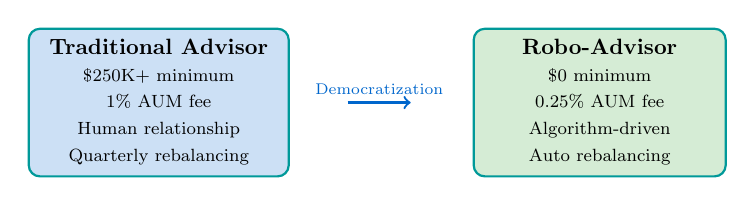
\begin{tikzpicture}[scale=0.8, transform shape]
% Traditional vs Robo
\node[blockchain, minimum width=4cm, fill=dfblue!20] (trad) at (0,0) {
\begin{tabular}{c}
\textbf{Traditional Advisor}\\
\footnotesize \$250K+ minimum\\
\footnotesize 1\% AUM fee\\
\footnotesize Human relationship\\
\footnotesize Quarterly rebalancing
\end{tabular}
};

\node[blockchain, minimum width=4cm, fill=dfgreen!20] (robo) at (7,0) {
\begin{tabular}{c}
\textbf{Robo-Advisor}\\
\footnotesize \$0 minimum\\
\footnotesize 0.25\% AUM fee\\
\footnotesize Algorithm-driven\\
\footnotesize Auto rebalancing
\end{tabular}
};

\draw[thick, ->, dfblue] (3,0) -- (4,0) node[midway, above, font=\scriptsize] {Democratization};
\end{tikzpicture}
\end{center}

\vspace{3mm}
\textbf{How Robo-Advisors Work:}
\begin{enumerate}
\item User completes risk questionnaire
\item Algorithm builds diversified ETF portfolio
\item Automatic tax-loss harvesting
\item Continuous rebalancing
\end{enumerate}

\textbf{Impact:} Brought professional-grade portfolio management to anyone with \$5 to invest.
\end{frame}

% ==================== SLIDE 17: DeFi Yield ====================
\begin{frame}{Investing: DeFi Yield Strategies}
\begin{center}
\textbf{\Large Yearn Finance and Yield Aggregation}
\end{center}

\vspace{3mm}
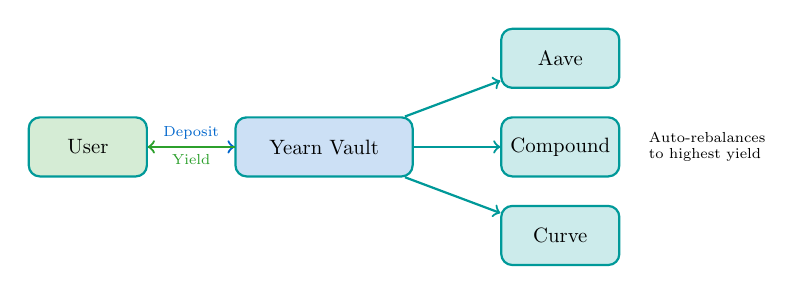
\begin{tikzpicture}[scale=0.75, transform shape]
% User deposits
\node[blockchain, minimum width=2cm, fill=dfgreen!20] (user) at (0,0) {User};
\node[blockchain, minimum width=3cm, fill=dfblue!20] (yearn) at (4,0) {Yearn Vault};

% Strategies
\node[blockchain, minimum width=2cm, fill=dfteal!20] (s1) at (8,1.5) {Aave};
\node[blockchain, minimum width=2cm, fill=dfteal!20] (s2) at (8,0) {Compound};
\node[blockchain, minimum width=2cm, fill=dfteal!20] (s3) at (8,-1.5) {Curve};

% Arrows
\draw[thick, ->, dfblue] (user) -- (yearn) node[midway, above, font=\scriptsize] {Deposit};
\draw[thick, ->, dfteal] (yearn) -- (s1);
\draw[thick, ->, dfteal] (yearn) -- (s2);
\draw[thick, ->, dfteal] (yearn) -- (s3);

% Returns
\draw[thick, <-, dfgreen] (user) -- (yearn) node[midway, below, font=\scriptsize] {Yield};

\node[right of=s2, node distance=2.5cm, font=\scriptsize, text width=2cm, align=left] {Auto-rebalances to highest yield};
\end{tikzpicture}

\vspace{3mm}
\textbf{Key Innovation:} Automated strategies that optimize yield across multiple DeFi protocols. User deposits once, algorithm does the rest.

\begin{alertblock}{Risk Warning}
Smart contract risk, impermanent loss, protocol risk compound across strategies.
\end{alertblock}
\end{frame}

% ==================== SLIDE 18: Sector 5 - Insurance ====================
\begin{frame}{Sector 5: Insurance}
\begin{columns}[T]
\begin{column}{0.48\textwidth}
\textbf{What it covers:}
\begin{itemize}
\item InsurTech platforms
\item Parametric insurance
\item Peer-to-peer insurance
\item Embedded insurance
\item Smart contract coverage
\end{itemize}

\vspace{3mm}
\textbf{Key friction addressed:}\\
Cost, claims, access, transparency
\end{column}
\begin{column}{0.48\textwidth}
\textbf{FinTech examples:}
\begin{itemize}
\item Lemonade, Root
\item Oscar, Hippo
\item Metromile
\end{itemize}

\vspace{3mm}
\textbf{Crypto examples:}
\begin{itemize}
\item Nexus Mutual
\item Cover Protocol
\item InsurAce
\end{itemize}
\end{column}
\end{columns}

\vspace{3mm}
\begin{block}{Coming in Day 5}
Insurance technology, parametric insurance, and DeFi coverage.
\end{block}
\end{frame}

% ==================== SLIDE 19: InsurTech Innovation ====================
\begin{frame}{Insurance: InsurTech Innovation}
\begin{columns}[T]
\begin{column}{0.48\textwidth}
\textbf{Traditional Insurance Pain Points:}
\begin{itemize}
\item Slow claims processing (weeks)
\item Opaque pricing
\item High overhead costs
\item Adversarial relationship
\item One-size-fits-all products
\end{itemize}

\vspace{3mm}
\textbf{InsurTech Solutions:}
\begin{itemize}
\item AI-powered instant claims
\item Transparent algorithms
\item Digital-first operations
\item Behavioral data pricing
\end{itemize}
\end{column}
\begin{column}{0.48\textwidth}
\textbf{Case Study: Lemonade}
\begin{itemize}
\item 90-second sign-up
\item 3-minute claims (AI-powered)
\item Giveback model: unused premiums to charity
\item \$50M+ in claims paid via bot
\end{itemize}

\vspace{3mm}
\textbf{Parametric Insurance:}
\begin{itemize}
\item Payout triggered by event, not claim
\item Example: Flight delay = automatic payment
\item Eliminates claims process entirely
\end{itemize}
\end{column}
\end{columns}
\end{frame}

% ==================== SLIDE 20: DeFi Insurance ====================
\begin{frame}{Insurance: DeFi Smart Contract Coverage}
\begin{center}
\textbf{\Large Nexus Mutual: Decentralized Insurance}
\end{center}

\vspace{3mm}
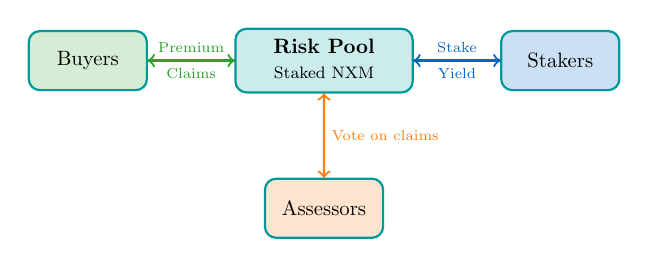
\begin{tikzpicture}[scale=0.75, transform shape]
% Pool structure
\node[blockchain, minimum width=3cm, fill=dfteal!20] (pool) at (4,0) {
\begin{tabular}{c}
\textbf{Risk Pool}\\
\footnotesize Staked NXM
\end{tabular}
};

% Members
\node[blockchain, minimum width=2cm, fill=dfgreen!20] (buy) at (0,0) {Buyers};
\node[blockchain, minimum width=2cm, fill=dfblue!20] (stake) at (8,0) {Stakers};

% Flows
\draw[thick, ->, dfgreen] (buy) -- (pool) node[midway, above, font=\scriptsize] {Premium};
\draw[thick, <-, dfgreen] (buy) -- (pool) node[midway, below, font=\scriptsize] {Claims};

\draw[thick, ->, dfblue] (stake) -- (pool) node[midway, above, font=\scriptsize] {Stake};
\draw[thick, <-, dfblue] (stake) -- (pool) node[midway, below, font=\scriptsize] {Yield};

% Claims assessors
\node[blockchain, minimum width=2cm, fill=dforange!20] (assess) at (4,-2.5) {Assessors};
\draw[thick, <->, dforange] (pool) -- (assess) node[midway, right, font=\scriptsize] {Vote on claims};
\end{tikzpicture}

\vspace{3mm}
\textbf{What It Covers:}
\begin{itemize}
\item Smart contract failures (hacks, bugs)
\item Protocol insolvency
\item Oracle manipulation
\end{itemize}

\textbf{Paid Out:} \$15M+ in claims from DeFi exploits
\end{frame}

% ==================== SLIDE 21: Sector 6 - Banking ====================
\begin{frame}{Sector 6: Banking Infrastructure}
\begin{columns}[T]
\begin{column}{0.48\textwidth}
\textbf{What it covers:}
\begin{itemize}
\item Neobanks
\item Banking-as-a-Service (BaaS)
\item Core banking platforms
\item Open banking APIs
\item Account aggregation
\end{itemize}

\vspace{3mm}
\textbf{Key friction addressed:}\\
Fees, UX, bundling, access
\end{column}
\begin{column}{0.48\textwidth}
\textbf{FinTech examples:}
\begin{itemize}
\item Chime, N26, Revolut
\item Plaid, MX, Yodlee
\item Synapse, Unit, Treasury Prime
\end{itemize}

\vspace{3mm}
\textbf{Crypto parallels:}
\begin{itemize}
\item Self-custody wallets
\item Account abstraction (ERC-4337)
\item On-chain identity
\end{itemize}
\end{column}
\end{columns}

\vspace{3mm}
\begin{alertblock}{Neobank Examples You Might Know}
\textbf{No branches:} Revolut, N26, Chime, Monzo -- banks with no physical branches, app-only\\
\textbf{vs. Traditional:} Deutsche Bank, Chase, HSBC with thousands of branches worldwide
\end{alertblock}

\vspace{2mm}
\begin{block}{Coming in Day 2}
Platform finance, open banking, and the future of banking infrastructure.
\end{block}
\end{frame}

% ==================== SLIDE 22: Neobanks ====================
\begin{frame}{Banking: Neobanks}
\begin{center}
\textbf{\Large Mobile-First Digital Banks}
\end{center}

\vspace{3mm}
\begin{columns}[T]
\begin{column}{0.48\textwidth}
\textbf{What Makes a Neobank:}
\begin{itemize}
\item No physical branches
\item Mobile app as primary interface
\item Lower fees (no branch overhead)
\item Modern UX design
\item Rapid feature deployment
\end{itemize}

\vspace{3mm}
\textbf{Major Players:}
\begin{itemize}
\item \textbf{US:} Chime (14M+ users)
\item \textbf{Europe:} N26, Revolut
\item \textbf{Brazil:} Nubank (70M+ users)
\item \textbf{UK:} Monzo, Starling
\end{itemize}
\end{column}
\begin{column}{0.48\textwidth}
\textbf{How They Work:}
\begin{enumerate}
\item Partner bank holds deposits (FDIC insured)
\item Neobank provides UX layer
\item Revenue from interchange, premium tiers
\item Lower CAC through viral growth
\end{enumerate}

\vspace{3mm}
\begin{block}{Key Insight}
Neobanks unbundle traditional banks, offering better UX for specific use cases while still using regulated banking infrastructure.
\end{block}
\end{column}
\end{columns}
\end{frame}

% ==================== SLIDE 23: Banking-as-a-Service ====================
\begin{frame}{Banking: BaaS Infrastructure}
\begin{center}
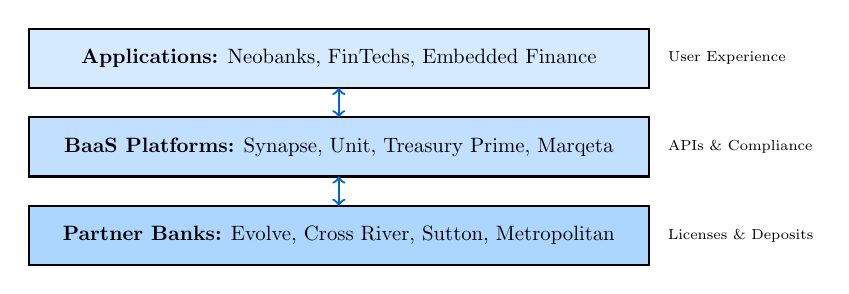
\begin{tikzpicture}[scale=0.75, transform shape]
% Layers
\draw[thick, fill=dflightblue4] (-0.5,3) rectangle (10,4);
\node at (4.75,3.5) {\textbf{Applications:} Neobanks, FinTechs, Embedded Finance};

\draw[thick, fill=dflightblue3] (-0.5,1.5) rectangle (10,2.5);
\node at (4.75,2) {\textbf{BaaS Platforms:} Synapse, Unit, Treasury Prime, Marqeta};

\draw[thick, fill=dflightblue2] (-0.5,0) rectangle (10,1);
\node at (4.75,0.5) {\textbf{Partner Banks:} Evolve, Cross River, Sutton, Metropolitan};

% Arrows
\draw[thick, <->, dfblue] (4.75,3) -- (4.75,2.5);
\draw[thick, <->, dfblue] (4.75,1.5) -- (4.75,1);

% Labels
\node[right] at (10.2,3.5) {\scriptsize User Experience};
\node[right] at (10.2,2) {\scriptsize APIs \& Compliance};
\node[right] at (10.2,0.5) {\scriptsize Licenses \& Deposits};
\end{tikzpicture}
\end{center}

\vspace{3mm}
\textbf{What BaaS Enables:}
\begin{itemize}
\item Any company can offer banking features via API
\item No bank charter required
\item Compliance handled by BaaS platform
\item Examples: Shopify Balance, Uber driver accounts, company expense cards
\end{itemize}
\end{frame}

% ==================== SLIDE 24: Infrastructure Layer ====================
\begin{frame}{Infrastructure Layer}
\begin{center}
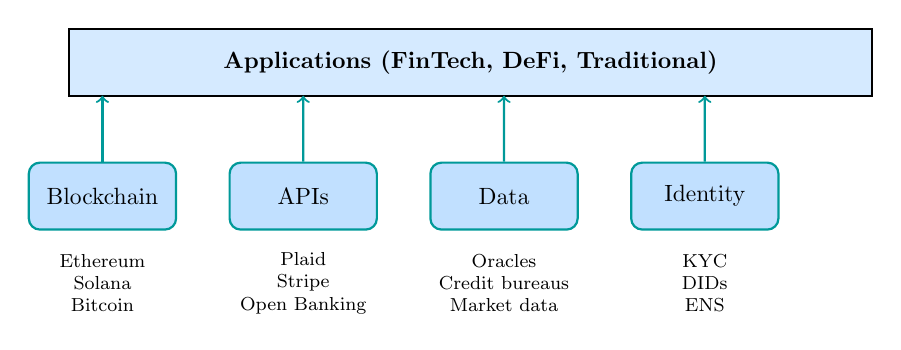
\begin{tikzpicture}[scale=0.85, transform shape]
% Infrastructure components
\node (blockchain) [blockchain, minimum width=2.2cm] {Blockchain};
\node (apis) [blockchain, right of=blockchain, node distance=3cm, minimum width=2.2cm] {APIs};
\node (data) [blockchain, right of=apis, node distance=3cm, minimum width=2.2cm] {Data};
\node (identity) [blockchain, right of=data, node distance=3cm, minimum width=2.2cm] {Identity};

% Applications layer above
\draw[thick, fill=dflightblue4] (-0.5,1.5) rectangle (11.5,2.5);
\node at (5.5,2) {\textbf{Applications (FinTech, DeFi, Traditional)}};

% Arrows up
\draw[->, thick, dfteal] (blockchain) -- ++(0,1.5);
\draw[->, thick, dfteal] (apis) -- ++(0,1.5);
\draw[->, thick, dfteal] (data) -- ++(0,1.5);
\draw[->, thick, dfteal] (identity) -- ++(0,1.5);

% Examples below each
\node[below of=blockchain, node distance=1.3cm, font=\footnotesize, text width=2cm, align=center] {Ethereum\\Solana\\Bitcoin};
\node[below of=apis, node distance=1.3cm, font=\footnotesize, text width=2cm, align=center] {Plaid\\Stripe\\Open Banking};
\node[below of=data, node distance=1.3cm, font=\footnotesize, text width=2cm, align=center] {Oracles\\Credit bureaus\\Market data};
\node[below of=identity, node distance=1.3cm, font=\footnotesize, text width=2cm, align=center] {KYC\\DIDs\\ENS};
\end{tikzpicture}
\end{center}

\vspace{3mm}
\textbf{Key insight:} All applications build on shared infrastructure.\\
Understanding the infrastructure helps you understand what's possible.
\end{frame}

% ==================== SLIDE 25: Infrastructure - Blockchain ====================
\begin{frame}{Infrastructure: Blockchain Networks}
\begin{columns}[T]
\begin{column}{0.48\textwidth}
\textbf{Purpose in Digital Finance:}
\begin{itemize}
\item Settlement layer for value transfer
\item Trustless execution environment
\item Immutable record keeping
\item Programmable money (smart contracts)
\end{itemize}

\vspace{3mm}
\textbf{Key Networks:}
\begin{itemize}
\item \textbf{Bitcoin:} Store of value, payments
\item \textbf{Ethereum:} Smart contracts, DeFi
\item \textbf{Solana:} High-speed transactions
\item \textbf{Layer 2s:} Scaling solutions
\end{itemize}
\end{column}
\begin{column}{0.48\textwidth}
\textbf{Why It Matters:}
\begin{itemize}
\item Enables trustless, permissionless finance
\item 24/7/365 operation
\item Global by default
\item Composable building blocks
\end{itemize}

\vspace{3mm}
\begin{block}{Trade-off}
\textbf{Decentralization} vs. \textbf{Scalability} vs. \textbf{Security}\\
Different chains make different choices.
\end{block}
\end{column}
\end{columns}
\end{frame}

% ==================== SLIDE 26: Infrastructure - APIs ====================
\begin{frame}{Infrastructure: APIs and Open Banking}
\begin{columns}[T]
\begin{column}{0.48\textwidth}
\textbf{What APIs Enable:}
\begin{itemize}
\item Connect apps to bank data
\item Initiate payments programmatically
\item Verify identity and accounts
\item Aggregate financial data
\end{itemize}

\vspace{2mm}
\begin{alertblock}{Simple Example}
\textbf{How does Uber show your bank balance without being your bank?} APIs -- secure data pipes between apps. Uber uses Plaid API to connect to your bank safely.
\end{alertblock}

\vspace{3mm}
\textbf{Key Players:}
\begin{itemize}
\item \textbf{Plaid:} Account connectivity
\item \textbf{Stripe:} Payment processing
\item \textbf{MX:} Financial data
\item \textbf{Yodlee:} Account aggregation
\end{itemize}
\end{column}
\begin{column}{0.48\textwidth}
\textbf{Open Banking Regulation:}
\begin{itemize}
\item PSD2 (Europe): Mandated API access
\item US: Market-driven (Plaid, etc.)
\item UK: Open Banking Standard
\item Australia: CDR framework
\end{itemize}

\vspace{3mm}
\begin{block}{Impact}
APIs are the ``picks and shovels'' of FinTech. Every major FinTech app relies on API infrastructure.
\end{block}
\end{column}
\end{columns}
\end{frame}

% ==================== SLIDE 27: Infrastructure - Data and Identity ====================
\begin{frame}{Infrastructure: Data and Identity}
\begin{columns}[T]
\begin{column}{0.48\textwidth}
\textbf{Data Infrastructure:}
\begin{itemize}
\item \textbf{Oracles:} Bring off-chain data on-chain
\item \textbf{Credit bureaus:} Traditional scoring
\item \textbf{Market data:} Prices, rates, feeds
\item \textbf{Alternative data:} Social, behavioral
\end{itemize}

\vspace{3mm}
\textbf{Key Oracle: Chainlink}
\begin{itemize}
\item Price feeds for DeFi
\item \$75B+ TVL secured
\item Critical infrastructure
\end{itemize}
\end{column}
\begin{column}{0.48\textwidth}
\textbf{Identity Infrastructure:}
\begin{itemize}
\item \textbf{KYC/AML:} Regulatory compliance
\item \textbf{DIDs:} Decentralized identifiers
\item \textbf{ENS:} Ethereum Name Service
\item \textbf{Verifiable credentials:} Portable identity
\end{itemize}

\vspace{3mm}
\begin{alertblock}{The Identity Challenge}
How do we enable privacy while meeting regulatory requirements? This remains an unsolved problem at scale.
\end{alertblock}
\end{column}
\end{columns}
\end{frame}

% ==================== SLIDE 28: Emerging Categories ====================
\begin{frame}{Emerging Categories}
\begin{columns}[T]
\begin{column}{0.48\textwidth}
\textbf{Tokenization:}
\begin{itemize}
\item Real estate tokens
\item Art and collectibles
\item Carbon credits
\item Securities tokenization
\end{itemize}

\vspace{3mm}
\textbf{DAOs:}
\begin{itemize}
\item Decentralized governance
\item Treasury management
\item Collective investing
\end{itemize}
\end{column}
\begin{column}{0.48\textwidth}
\textbf{CBDCs:}
\begin{itemize}
\item Central Bank Digital Currencies
\item Government-issued digital money
\item Wholesale vs. retail
\end{itemize}

\vspace{2mm}
\begin{alertblock}{Simple Framing}
Think of CBDC as government-issued digital cash -- like having euro notes, but digital and issued directly by the central bank instead of commercial banks.
\end{alertblock}

\vspace{3mm}
\textbf{AI + Finance:}
\begin{itemize}
\item Algorithmic credit scoring
\item Fraud detection
\item Automated advising
\item Predictive analytics
\end{itemize}
\end{column}
\end{columns}

\vspace{3mm}
\begin{block}{Coming in Days 5 \& 6}
Tokenization, DAOs, CBDCs, and the future of digital finance.
\end{block}
\end{frame}

% ==================== SLIDE 29: Discussion - Convergence ====================
\begin{frame}{Discussion: The Convergence Trend}
\begin{center}
\textbf{\Large The Lines Are Blurring}
\end{center}

\vspace{3mm}
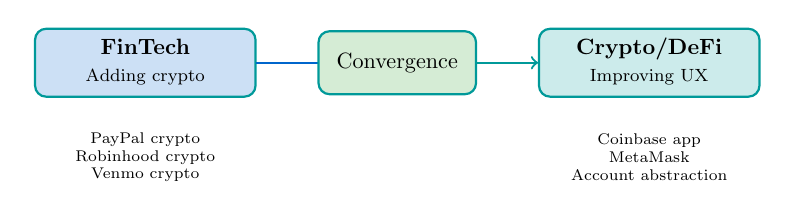
\begin{tikzpicture}[scale=0.8, transform shape]
% FinTech side
\node[blockchain, minimum width=3.5cm, fill=dfblue!20] (fintech) at (0,0) {
\begin{tabular}{c}
\textbf{FinTech}\\
\footnotesize Adding crypto
\end{tabular}
};

% Crypto side
\node[blockchain, minimum width=3.5cm, fill=dfteal!20] (crypto) at (8,0) {
\begin{tabular}{c}
\textbf{Crypto/DeFi}\\
\footnotesize Improving UX
\end{tabular}
};

% Convergence arrows
\draw[thick, ->, dfblue] (fintech) -- (4,0);
\draw[thick, <-, dfteal] (crypto) -- (4,0);

% Center overlap
\node[blockchain, minimum width=2.5cm, fill=dfgreen!20] at (4,0) {Convergence};

% Examples
\node[below of=fintech, node distance=1.5cm, font=\scriptsize, text width=3.5cm, align=center] {PayPal crypto\\Robinhood crypto\\Venmo crypto};
\node[below of=crypto, node distance=1.5cm, font=\scriptsize, text width=3.5cm, align=center] {Coinbase app\\MetaMask\\Account abstraction};
\end{tikzpicture}

\vspace{3mm}
\textbf{Discussion Questions:}
\begin{itemize}
\item Will the distinction between FinTech and DeFi disappear?
\item What determines which approach wins for a given use case?
\item How should traditional banks respond?
\end{itemize}
\end{frame}

% ==================== SLIDE 30: Application Exercise ====================
\begin{frame}{Application: Mapping Innovations}
\begin{center}
\textbf{\Large Exercise: Place These in the Landscape}
\end{center}

\vspace{3mm}
\begin{columns}[T]
\begin{column}{0.48\textwidth}
\textbf{Innovation Examples:}
\begin{enumerate}
\item Wise (cross-border payments)
\item Aave (lending protocol)
\item Robinhood (stock trading)
\item Lemonade (insurance)
\item Chime (neobank)
\item Yearn Finance (yield)
\end{enumerate}
\end{column}
\begin{column}{0.48\textwidth}
\textbf{For Each, Identify:}
\begin{itemize}
\item Which sector?
\item FinTech or Crypto/DeFi?
\item What friction does it address?
\item What infrastructure does it use?
\item Who benefits most?
\end{itemize}
\end{column}
\end{columns}

\vspace{5mm}
\begin{block}{Goal}
Practice using the landscape framework to quickly categorize and understand any digital finance innovation you encounter.
\end{block}
\end{frame}

% ==================== SLIDE 31: Executive Summary ====================
\begin{frame}{Executive Summary}
\begin{center}
\textbf{\Large Key Takeaways from the Landscape}
\end{center}

\vspace{3mm}
\begin{columns}[T]
\begin{column}{0.48\textwidth}
\textbf{The Six Sectors:}
\begin{enumerate}
\item \textbf{Payments:} Moving money
\item \textbf{Lending:} Access to credit
\item \textbf{Trading:} Market access
\item \textbf{Investing:} Wealth building
\item \textbf{Insurance:} Risk management
\item \textbf{Banking:} Account infrastructure
\end{enumerate}

\vspace{3mm}
\textbf{Two Philosophies:}
\begin{itemize}
\item FinTech: Better UX, existing rails
\item Crypto/DeFi: New rails, new rules
\end{itemize}
\end{column}
\begin{column}{0.48\textwidth}
\textbf{Shared Infrastructure:}
\begin{itemize}
\item Blockchain networks
\item APIs and open banking
\item Data systems and oracles
\item Identity infrastructure
\end{itemize}

\vspace{3mm}
\begin{alertblock}{Central Question}
For any given use case: Should we improve existing infrastructure or build new infrastructure?
\end{alertblock}
\end{column}
\end{columns}
\end{frame}

% ==================== SLIDE 32: Concept Map ====================
\begin{frame}{Concept Map: The Digital Finance Ecosystem}
\begin{center}
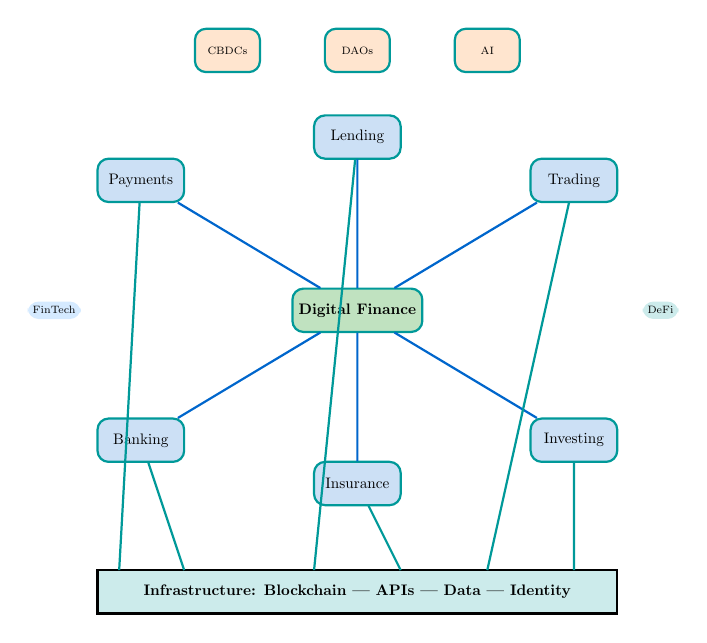
\begin{tikzpicture}[scale=0.55, transform shape]
% Central node
\node[blockchain, minimum width=3cm, fill=dfgreen!30] (center) at (5,0) {\textbf{Digital Finance}};

% Sector nodes arranged in circle
\node[blockchain, minimum width=2cm, fill=dfblue!20] (pay) at (0,3) {Payments};
\node[blockchain, minimum width=2cm, fill=dfblue!20] (lend) at (5,4) {Lending};
\node[blockchain, minimum width=2cm, fill=dfblue!20] (trade) at (10,3) {Trading};
\node[blockchain, minimum width=2cm, fill=dfblue!20] (invest) at (10,-3) {Investing};
\node[blockchain, minimum width=2cm, fill=dfblue!20] (ins) at (5,-4) {Insurance};
\node[blockchain, minimum width=2cm, fill=dfblue!20] (bank) at (0,-3) {Banking};

% Connect to center
\draw[thick, dfblue] (center) -- (pay);
\draw[thick, dfblue] (center) -- (lend);
\draw[thick, dfblue] (center) -- (trade);
\draw[thick, dfblue] (center) -- (invest);
\draw[thick, dfblue] (center) -- (ins);
\draw[thick, dfblue] (center) -- (bank);

% Infrastructure bar at bottom
\draw[thick, fill=dfteal!20] (-1,-6) rectangle (11,-7);
\node at (5,-6.5) {\textbf{Infrastructure: Blockchain | APIs | Data | Identity}};

% Connect sectors to infrastructure
\draw[thick, dfteal] (pay) -- (-0.5,-6);
\draw[thick, dfteal] (bank) -- (1,-6);
\draw[thick, dfteal] (lend) -- (4,-6);
\draw[thick, dfteal] (ins) -- (6,-6);
\draw[thick, dfteal] (trade) -- (8,-6);
\draw[thick, dfteal] (invest) -- (10,-6);

% Philosophy labels
\node[fill=dflightblue4, rounded corners] at (-2,0) {\scriptsize FinTech};
\node[fill=dfteal!20, rounded corners] at (12,0) {\scriptsize DeFi};

% Emerging categories
\node[blockchain, minimum width=1.5cm, fill=dforange!20, font=\scriptsize] at (2,6) {CBDCs};
\node[blockchain, minimum width=1.5cm, fill=dforange!20, font=\scriptsize] at (5,6) {DAOs};
\node[blockchain, minimum width=1.5cm, fill=dforange!20, font=\scriptsize] at (8,6) {AI};
\end{tikzpicture}
\end{center}
\end{frame}

% ==================== SLIDE 33: Key Terms (Part 1) ====================
\begin{frame}{Key Terms and Definitions (Part 1)}
\begin{columns}[T]
\begin{column}{0.48\textwidth}
\textbf{Sectors:}
\begin{description}
\item[Neobank] Digital-first bank with no physical branches
\item[BNPL] Buy Now, Pay Later installment lending
\item[Robo-advisor] Algorithm-driven investment management
\item[InsurTech] Technology-enabled insurance innovation
\item[DEX] Decentralized exchange using smart contracts
\item[CEX] Centralized exchange with custodial model
\end{description}
\end{column}
\begin{column}{0.48\textwidth}
\textbf{Business Models:}
\begin{description}
\item[BaaS] Banking-as-a-Service API platforms
\item[Embedded Finance] Financial services in non-financial apps
\item[Open Banking] API access to bank data (regulated)
\item[AMM] Automated Market Maker for DEX trading
\item[Yield Aggregator] Auto-optimizing DeFi returns
\end{description}
\end{column}
\end{columns}
\end{frame}

% ==================== SLIDE 34: Key Terms (Part 2) ====================
\begin{frame}{Key Terms and Definitions (Part 2)}
\begin{columns}[T]
\begin{column}{0.48\textwidth}
\textbf{Infrastructure:}
\begin{description}
\item[Oracle] Service bringing off-chain data on-chain
\item[KYC] Know Your Customer identity verification
\item[DID] Decentralized Identifier for portable identity
\item[ENS] Ethereum Name Service (human-readable addresses)
\item[Layer 2] Scaling solution built on top of Layer 1
\end{description}
\end{column}
\begin{column}{0.48\textwidth}
\textbf{Emerging Concepts:}
\begin{description}
\item[Tokenization] Representing assets as blockchain tokens
\item[DAO] Decentralized Autonomous Organization
\item[CBDC] Central Bank Digital Currency
\item[Composability] ``Money legos'' -- combining DeFi protocols
\item[Account Abstraction] Smart contract wallets (ERC-4337)
\end{description}
\end{column}
\end{columns}

\vspace{5mm}
\begin{block}{Why Terms Matter}
The landscape has its own vocabulary. Mastering these terms lets you navigate industry discussions, research, and opportunities.
\end{block}
\end{frame}

% ==================== SLIDE 35: Common Misconceptions ====================
\begin{frame}{Common Misconceptions}
\begin{center}
\textbf{\Large Myths vs. Reality in Digital Finance}
\end{center}

\vspace{3mm}
\begin{columns}[T]
\begin{column}{0.48\textwidth}
\textbf{Myth 1:} ``FinTech and DeFi are competing''\\
\textcolor{dfgreen}{\textbf{Reality:}} They often complement each other. Many companies use both approaches.

\vspace{3mm}
\textbf{Myth 2:} ``Neobanks are replacing traditional banks''\\
\textcolor{dfgreen}{\textbf{Reality:}} Most neobanks partner WITH banks for licensing and deposits.

\vspace{3mm}
\textbf{Myth 3:} ``DeFi is only for speculation''\\
\textcolor{dfgreen}{\textbf{Reality:}} DeFi includes lending, insurance, and infrastructure -- not just trading.
\end{column}
\begin{column}{0.48\textwidth}
\textbf{Myth 4:} ``Blockchain = cryptocurrency''\\
\textcolor{dfgreen}{\textbf{Reality:}} Blockchain is infrastructure; crypto is one application.

\vspace{3mm}
\textbf{Myth 5:} ``Digital finance is unregulated''\\
\textcolor{dfgreen}{\textbf{Reality:}} FinTech is heavily regulated; DeFi regulation is evolving rapidly.

\vspace{3mm}
\textbf{Myth 6:} ``The landscape is fixed''\\
\textcolor{dfgreen}{\textbf{Reality:}} New categories emerge constantly. The map evolves.
\end{column}
\end{columns}
\end{frame}

% ==================== SLIDE 36: Self-Assessment Question 1 ====================
\begin{frame}{Self-Assessment: Question 1}
\begin{block}{Quiz Question (ID: 3)}
Which FinTech company category represents mobile-first digital banks with no physical branches?
\end{block}

\vspace{3mm}
\begin{enumerate}[A.]
\item Payment processors
\item Neobanks
\item Robo-advisors
\item InsurTech
\end{enumerate}

\vspace{5mm}
\pause
\textbf{Answer: B -- Neobanks}

\vspace{3mm}
\textbf{Explanation:} Neobanks (like Chime, N26, Revolut, and Nubank) are digital-first banks that operate primarily or exclusively through mobile apps without physical branch networks. They still use traditional banking infrastructure and are licensed banks, but offer better user experience, lower fees, and modern features compared to traditional banks.
\end{frame}

% ==================== SLIDE 37: Self-Assessment Questions 2 & 3 ====================
\begin{frame}{Self-Assessment: Questions 2 \& 3}
\begin{block}{Quiz Question (ID: 8)}
What is the primary friction that payment sector innovations address?
\end{block}
\begin{enumerate}[A.]
\item Investment returns
\item \textbf{Speed, cost, and convenience of money movement}
\item Insurance claims processing
\item Credit scoring accuracy
\end{enumerate}
\textbf{Answer: B} -- Payment innovations target speed (3-5 day international transfers), cost (especially cross-border), and convenience (limited hours, geographic restrictions).

\vspace{5mm}
\begin{block}{Quiz Question (ID: 16)}
What is the convergence trend described in the landscape overview?
\end{block}
\begin{enumerate}[A.]
\item All financial companies are becoming exactly the same
\item \textbf{FinTech adds crypto features while crypto improves UX, blurring lines}
\item Traditional banks are completely disappearing
\item Cash is being eliminated worldwide
\end{enumerate}
\textbf{Answer: B} -- Despite convergence, the underlying philosophical differences remain distinct.
\end{frame}

% ==================== SLIDE 38: What's Next ====================
\begin{frame}{Looking Ahead: Day 2}
\begin{center}
\textbf{\Large Platform Finance: How FinTech Reshapes Financial Services}
\end{center}

\vspace{5mm}
\textbf{We'll explore:}
\begin{itemize}
\item How platforms create value through network effects
\item Open banking and API-based innovation
\item Neobanks and the unbundling of finance
\item Platform business models
\end{itemize}

\vspace{5mm}
\textbf{Preparation:}
\begin{itemize}
\item Think: What financial apps do you use daily?
\item Optional: Read about payment rails (ACH, SWIFT, card networks)
\item Consider: Which sectors interest you most for deeper exploration?
\end{itemize}

\vspace{3mm}
\begin{block}{Preview}
Day 2 goes deep on the FinTech side of the landscape -- how platforms, APIs, and network effects are transforming traditional financial services.
\end{block}
\end{frame}

% ==================== SLIDE 39: Resources ====================
\begin{frame}{Resources}
\textbf{Further Reading:}
\begin{itemize}
\item Nakamoto, S. (2008). ``Bitcoin: A Peer-to-Peer Electronic Cash System''
\item World Bank Global Findex Database
\item BIS Papers on payments and digital currencies
\item CB Insights FinTech 250 annual report
\end{itemize}

\vspace{3mm}
\textbf{Industry Sources:}
\begin{itemize}
\item DeFi Llama (TVL tracking): \texttt{defillama.com}
\item The Block (industry news): \texttt{theblock.co}
\item Fintech Nexus (conferences): \texttt{fintechnexus.com}
\end{itemize}

\vspace{3mm}
\textbf{Concepts to Review:}
\begin{itemize}
\item The six sectors of digital finance
\item Infrastructure layer components
\item FinTech vs. Crypto/DeFi distinction
\item Emerging categories: tokenization, DAOs, CBDCs, AI
\end{itemize}
\end{frame}

% ==================== SLIDE 40: Questions ====================
\begin{frame}{Questions?}
\begin{center}
\textbf{\LARGE Questions and Discussion}

\vspace{10mm}
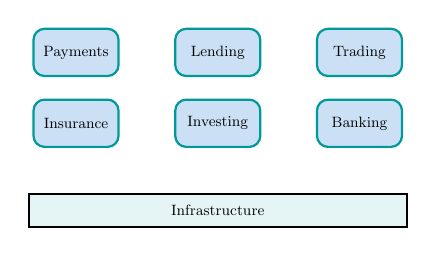
\begin{tikzpicture}[scale=0.6, transform shape]
% Recreate mini landscape
\node[blockchain, minimum width=1.8cm, fill=dfblue!20] (p) at (0,1.5) {\small Payments};
\node[blockchain, minimum width=1.8cm, fill=dfblue!20] (l) at (3,1.5) {\small Lending};
\node[blockchain, minimum width=1.8cm, fill=dfblue!20] (t) at (6,1.5) {\small Trading};
\node[blockchain, minimum width=1.8cm, fill=dfblue!20] (i) at (0,0) {\small Insurance};
\node[blockchain, minimum width=1.8cm, fill=dfblue!20] (inv) at (3,0) {\small Investing};
\node[blockchain, minimum width=1.8cm, fill=dfblue!20] (b) at (6,0) {\small Banking};
\draw[thick, fill=dfteal!10] (-1,-1.5) rectangle (7,-2.2);
\node at (3,-1.85) {\small Infrastructure};
\end{tikzpicture}

\vspace{10mm}
\textbf{Contact:} Joerg Osterrieder\\
\textbf{Topic:} T1.4 -- Landscape Overview
\end{center}
\end{frame}

\end{document}
